\documentclass[border=10pt]{standalone}
\usepackage{pgfplots}
\pgfplotsset{compat=1.17}
\begin{document}
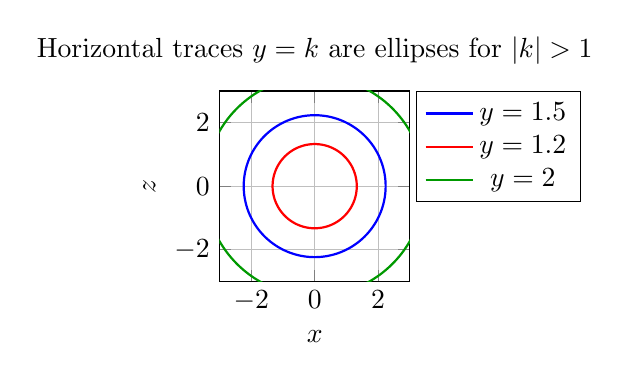
\begin{tikzpicture}
\begin{axis}[
    width=12cm, height=4cm,
    axis equal image,
    xmin=-3, xmax=3, ymin=-3, ymax=3,
    xlabel=$x$, ylabel=$z$,
    grid=both,
    title={Horizontal traces $y=k$ are ellipses for $|k|>1$},
    legend pos=outer north east
]
\def\yval{1.5}
\addplot[blue, thick, domain=0:360, samples=200, variable=\t]
    ({2*sqrt(\yval^2-1)*cos(\t)}, {2*sqrt(\yval^2-1)*sin(\t)});
\def\yvalb{1.2}
\addplot[red, thick, domain=0:360, samples=200, variable=\t]
    ({2*sqrt(\yvalb^2-1)*cos(\t)}, {2*sqrt(\yvalb^2-1)*sin(\t)});
\def\yvalc{2}
\addplot[green!60!black, thick, domain=0:360, samples=200, variable=\t]
    ({2*sqrt(\yvalc^2-1)*cos(\t)}, {2*sqrt(\yvalc^2-1)*sin(\t)});
\legend{$y=1.5$,$y=1.2$,$y=2$}
\end{axis}
\end{tikzpicture}
\end{document}
